\documentclass[12pt]{article}

%Modelo de pré-projeto para o curso de Tecnologia em Sistemas para Internet
%do Instituto Federal de Educação, Ciência e Tecnologia do Tocantins.
%
%Modelo baseado nos templates da Sociedade Brasileira de Computação (SBC)
%Fonte: http://www.sbc.org.br
%
%@author Prof. Manoel Campos da Silva Filho - http://manoelcampos.com
%@version 1.1

%permitir o uso do comando \cellcolor para colorir células de uma tabela
\usepackage[table]{xcolor}

%\usepackage[brazil]{babel}   
\usepackage[brazilian]{babel}

%Permite definir o idioma da bibliografia
\usepackage[fixlanguage]{babelbib}

\usepackage{verbatim} 
% Pacote vertabim permite comentários em múltiplas linhas com:
\begin{comment}
linha 1
linha 2
linha N
\end{comment}

\usepackage[utf8]{inputenc}
%permite copiar texto acentuado no PDF gerado
\usepackage[T1]{fontenc}

\usepackage{sbc-template}
\usepackage{graphicx,url}

     
\sloppy

\title{Título do Projeto}

\author{Nome do Aluno\inst{1}, Nome do Professor Orientador\inst{1}}


\address{
  Coordenação de Informática\\
  Instituto Federal de Educação, Ciência e Tecnologia do Tocantins (IFTO)\\
  AE 301 Sul, Av. LO 05 S/N, Plano Diretor Sul, 77.021-090, Palmas-TO, Brasil
%\nextinstitute
%  Outro Departamento\\
%  Outra Instituição
\email{email.do.aluno@dominio, email.do.professor@ifto.edu.br}
}

\begin{document} 

\maketitle

\begin{abstract}
  Resumo em inglês
\end{abstract}
     
\begin{resumo} 
Aqui o aluno deve apresentar um resumo da sua proposta de TCC, que é o pré-projeto, descrevendo o que pretende desenvolver. O aluno deve tomar cuidado para que o resumo (e o abstract) não ultrapassem 10 linhas cada.
\end{resumo}

\section{Introdução} \label{sec:intro}

Nesta seção aluno deverá contextualizar sobre o tema do qual trata seu trabalho, introduzindo o leitor no assunto. 

%Observe que os parágrafos em latex são definidos apenas deixando-se
%uma linha em branco entre um e outro, como no Microsoft Word e similares.
Em seguida o aluno deve fazer uma breve apresentação do trabalho a ser desenvolvido, descrevendo o problema que ele pretende resolver ou estudar.

Em todo o texto, procure escrever frases curtas. Assim, vendo que um determinado trecho de uma frase já possui sentido completo, finalize o mesmo com ponto e inicia uma nova frase. Procure não deixar parágrafos muito longos.

Termos em inglês devem ser colocados em itálico ou entre aspas. A primeira vez que uma sigla for utilizada, primeiro deve-se incluir seu significado, seguido da sigla entre parênteses. Em momentos seguintes, pode-se utilizar apenas a sigla. 

É sugerido que o pré-projeto tenha entre 6 e 10 páginas.

%Especificar um label apropriado para cada seção e sub-seção criada
% (caso deseje referenciar tais seções durante o texto.
% Por exemplo, se tiver um texto como
% "Conforme apresentado na Seção 3",
% tal seção que você está referenciando
% precisa de um label (um nome) que é usado
% para fazer referência a ela no texto.
% Assim, digamos que você criou um \label{sec:arquitetura}
% Um texto que faça referência a tal seção ficaria assim:
% Conforme apresentado na Seção \ref{sec:arquitetura}

\section{Justificativa} \label{sec:justificativa}

Nesta seção o aluno deve justificar o desenvolvimento do projeto, apresentando os motivos pelos quais o mesmo será desenvolvido e que mostrem a viabilidade de seu desenvolvimento. 

Justificativas podem ser, por exemplo: a falta de algo semelhante ao que pretende desenvolver, ou que possua os mesmos recursos; o aprofundamento de pesquisa em determinada área, resultando na geração de artigos científicos a serem publicados para aumentar o acervo de material sobre o tema; a necessidade da instituição para a qual desenvolverá o projeto, etc.

\section{Proposta} \label{sec:proposta}
A partir daqui, o aluno pode dividir seu trabalho em seções e sub-seções numeradas, da forma como desejar, colocando os títulos adequados para cada uma. Obviamente, a numeração dos itens pré-definidos a seguir podem mudar de acordo com as seções que criar antes deles.

\section{Metodologia} \label{sec:metodologia}

Descrever como pretende desenvolver o projeto, definindo as fases para isto, como, por exemplo (para um projeto de software): levantamento bibliográfico e de trabalhos relacionados, levantamento de requisitos, análise e projeto, desenvolvimento e testes. No caso de projetos de software, o uso da UML deve ser incluído aqui na metodologia.

Cada item da metodologia pode ser feito em forma de parágrafo, explicando o que cada um representa e o que se pretende com a aplicação do mesmo. Um exemplo é apresentado no parágrafo a seguir.

Para desenvolvimento do projeto será feita pesquisa de outros sistemas existentes, como o Wish TV, em busca de suas características, recursos e falhas, para encontrar o que há de melhor na área e que pode ser aplicado à realidade brasileira. 

O levantamento bibliográfico é a busca de referências a serem usadas no projeto, devendo,  preferencialmente, ser baseada em livros e artigos científicos. Referências como Wikepedia e outros sites devem ser evitados, a não ser que sejam artigos em sites conceituados sobre o assunto do qual o projeto trata.

\section{Resultados Esperados} \label{sec:resultados}
Descrever o que se pretende alcançar ao final do desenvolvimento do projeto. Veja um exemplo no parágrafo a seguir.

	Ao final do desenvolvimento do projeto, pretende-se ter uma solução em software livre que possua uma interface gráfica amigável e intuitiva (sem a necessidade de realizar treinamentos longos com o usuário para uso do software), mostrando que os recursos desenvolvidos permitem um aumento de produtividade do usuário.
	
As Figuras \ref{fig:figura1} e \ref{fig:figura2} a seguir são apenas exemplos.

\begin{figure}[ht]
\centering
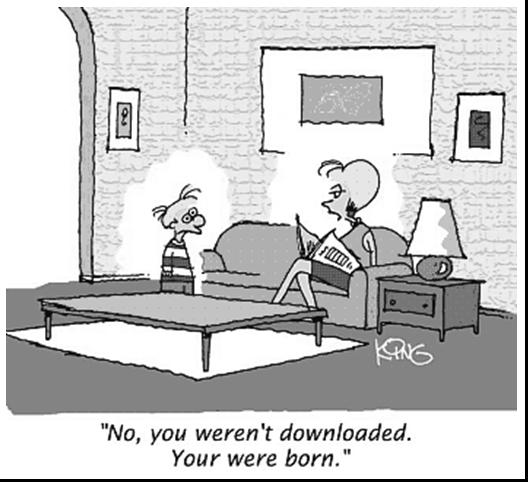
\includegraphics[width=.5\textwidth]{fig1.jpg}
\caption{Um exemplo de figura}
%Deve-se dar nomes apropriados aos labels das figuras. 
%Aqui foi utilizado figura1 apenas como exemplo
\label{fig:figura1}
\end{figure}

\begin{figure}[ht]
\centering
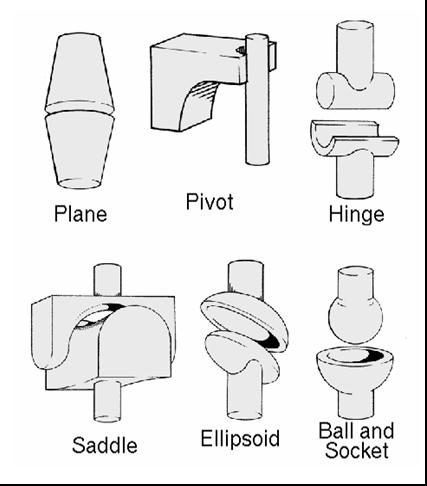
\includegraphics[width=.3\textwidth]{fig2.jpg}
\caption{Exempo de título de figura ocupando mais de uma linha de texto. Ao referenciar uma figura, deve-se usar a palavra Figura com inicial maiúscula, como pode ser visto no texto do parágrafo a seguir.}
%Deve-se dar nomes apropriados aos labels das figuras. 
%Aqui foi utilizado figura2 apenas como exemplo
\label{fig:figura2}
\end{figure}

Como pode ser observado nas Figuras \ref{fig:figura1} e \ref{fig:figura2}, a formatação do título da figura muda caso o texto tenha mais de uma linha.

A Tabela \ref{tab:tabela1} a seguir apresenta um exemplo de uso de tabelas.

\begin{center}
	\begin{tabular}{|p{3cm}|p{4cm}|p{6cm}|} %{|l|c|c|}
  \hline
		\textbf{Aplicação} & \textbf{Sem módulos implementados} & \textbf{Com módulos implementados} \\
  \hline
		Enquete/HTTP & 14 linhas de código\par5 funções  utilizadas diretamente & 
    5 linhas de código = 35\% do anterior\par1 função usada diretamente \\
  \hline
		Cotação do dólar/SOAP & 64 linhas de código\par5 funções  utilizadas diretamente & 
    15 linhas de código = 23\% do anterior
    \par(9 são parâmetros do WS) 1 função  usada diretamente \\
  \hline
	\end{tabular}
	\captionof{table}{Comparativo entre aplicações de TVD com e sem os módulos implementados}
	\label{tab:tabela1}
\end{center}
	
	
\section{Cronograma} \label{sec:cronograma}

Apresentar um cronograma das etapas de desenvolvimento do projeto, normalmente obtidas a partir da seção "Metodologia", que apresentou como o projeto será desenvolvido. A tabela abaixo apresenta um exemplo de cronograma dividido em semanas, para um período de 6 meses. O total de meses vai depender do prazo que o aluno tem. 

%Cria uma "variável" para definir a cor para pintar as células do cronograma
\newcommand{\corCronograma}{yellow}
\begin{center}
  %Definição da tabela e suas colunas. 
  %Pode-se usar o menu "Assistente" da ferramenta TeXstudio para criar tabelas facilmente.
	\begin{tabular}{|p{6cm}|p{1cm}|p{1cm}|p{1cm}|p{1cm}|p{1cm}|p{1cm}|}  %{|l|c|c|c|c|c|c|}
  \hline
    \multicolumn{7}{c}{2013}\\
  \hline
    %Títulos das colunas
  	\textbf{Etapas}&
  	\textbf{Jan}&
  	\textbf{Fev}&
  	\textbf{Mar}&
  	\textbf{Abr}&
  	\textbf{Mai}&
  	\textbf{Jun}
  	\\
  \hline
  Levantamento Bibliográfico &
  \cellcolor{\corCronograma} & & & & & 
  \\
  \hline
  Estudo das tecnologias envolvidas &
  & \cellcolor{\corCronograma} & & & & 
  \\
  \hline
  Levantamento de Requisitos &
  & & \cellcolor{\corCronograma} & & & 
  \\
  \hline
  Análise e Projeto &
  & & & \cellcolor{\corCronograma} & \cellcolor{\corCronograma} & \cellcolor{\corCronograma}
  \\
  \hline
  Desenvolvimento &
  & & & \cellcolor{\corCronograma} & \cellcolor{\corCronograma} & \cellcolor{\corCronograma}
  \\
  \hline
  Testes &
  & & & \cellcolor{\corCronograma} & \cellcolor{\corCronograma} & \cellcolor{\corCronograma}
  \\  
  \hline
	\end{tabular}
	\captionof{table}{Cronograma de execução do projeto}
	\label{tab:cronograma}
\end{center}

\section{Como Formatar as Referências} \label{sec:formatarReferencias}

As referências bibliográficas são formatadas automaticamente em LaTeX.
Tal formatação é definida pelo arquivo de estilo bibliográfico definido no comando \verb!\bibliographystyle{nome-arquivo-estilo-bibliografico}!. 

A seguir são apresentados exemplos de referências utilizando o comando \verb|\cite{referencia}| \cite{ncluasoap} \cite{tic2009}.

\selectbiblanguage{brazilian}
\bibliographystyle{sbc}
\bibliography{referencias}

\end{document}





